\documentclass[spanish, aspectratio=169]{beamer}
\usepackage[utf8]{inputenc}
\usepackage[spanish, mexico]{babel}
% Paquetes necesarios para incluir imágenes
\usepackage{graphicx}
\usepackage{caption}
\usepackage{subcaption}
\captionsetup{justification=centering}
% Bibliography
\usepackage[style=iso-authoryear, currentlang]{biblatex}
\addbibresource{../bibliography/referencias.bib}
\DeclareDelimFormat{nameyeardelim}{\addspace}
\usepackage{csquotes}

\usetheme{pittsburgh} 
%\usecolortheme{owl}
\setbeamertemplate{caption}[numbered]
\setbeamertemplate{sidebar right}{}
\setbeamertemplate{footline}{\hfill\usebeamertemplate***{navigation symbols}}
\setbeamercolor{footline}{fg=blue}

\addtobeamertemplate{navigation symbols}{}{%
    \usebeamerfont{footline}%
    \usebeamercolor[fg]{footline}%
    \hspace{1em}%
    \insertframenumber/\inserttotalframenumber
}

\title{Software para la Automatización de Programas de Gestión de Salud y Seguridad 
en el Trabajo conforme a la Norma Técnica de Seguridad 009}
\date{\today}
\author{Leonardo Achá Boiano}
\institute{Universidad Católica Boliviana ``San Pablo''}

\titlegraphic{
\includegraphics[height=.2\textheight]{../images/ucbLogo1.png}}

%----------------------------------------------------------------------------------
%----------------------------------------------------------------------------------

\begin{document}
\maketitle
  
%--------------------------------------------------------------------------------
\section{Introducción}
\begin{frame}[allowframebreaks]{Antecedentes}

  \textcite{cervantesdiagnostico} concluye que la mayoría de las leyes y regulaciones existentes en materia de seguridad y salud en el trabajo no se aplican debido a dos razones principales: 
  \begin{itemize}
    \item Obstáculos externos (como condiciones materiales, culturales y de acceso).
    \item Las entidades encargadas no disponen de las estructuras y recursos necesarios para supervisar su cumplimiento y sancionar las infracciones.
  \end{itemize}
  

  Mediante la Resolución Ministerial N° 1411/18, el 27 de diciembre de 2018, el Ministerio de Trabajo aprueba la Norma Técnica de Seguridad NTS-009/18.

  \framebreak

  \begin{columns}[T]
    \column{0.5\textwidth}
    \begin{figure}
        \centering
        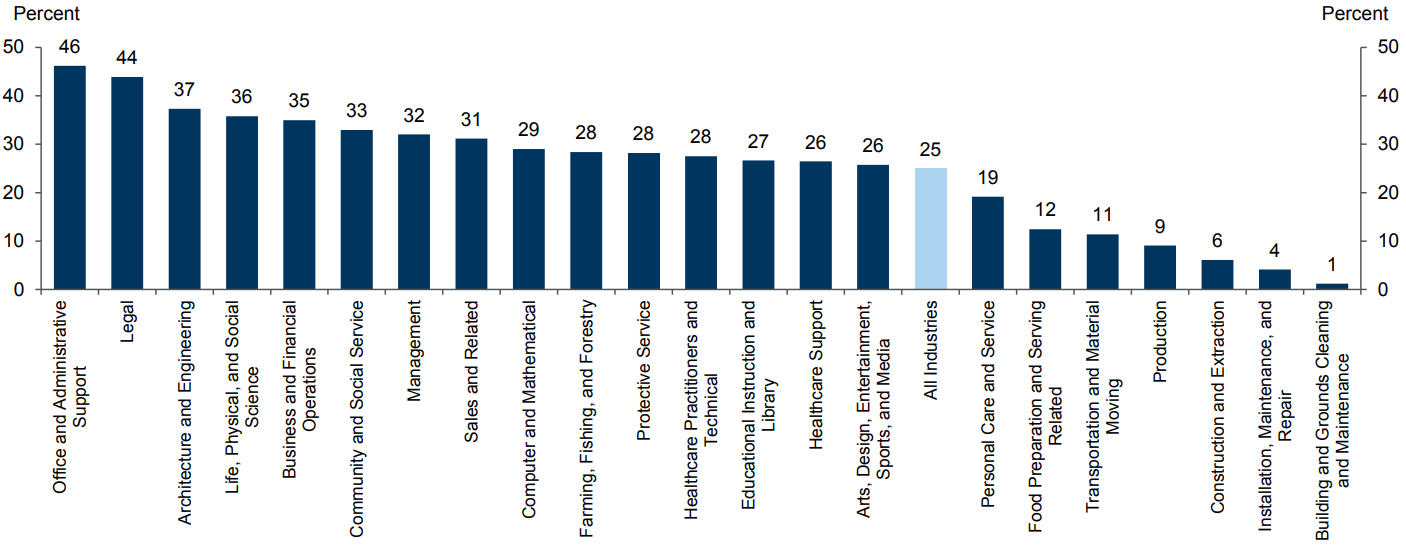
\includegraphics[width=\textwidth, height=.5\textheight]{../images/marcoref/share_of_industry_exposed_to_automation_ai.png}
        \caption{Porcentaje de la industria expuesta a la automatización por parte de la Inteligencia Artificial en Estados Unidos. Fuente: Goldman Sachs Global Investment Research (\citeyear{hatzius2023potentially}).}
        \label{fig:share_of_industry_exposed_to_automation_ai_gs}
    \end{figure}
    
    \column{0.5\textwidth}
    \begin{figure}
        \centering
        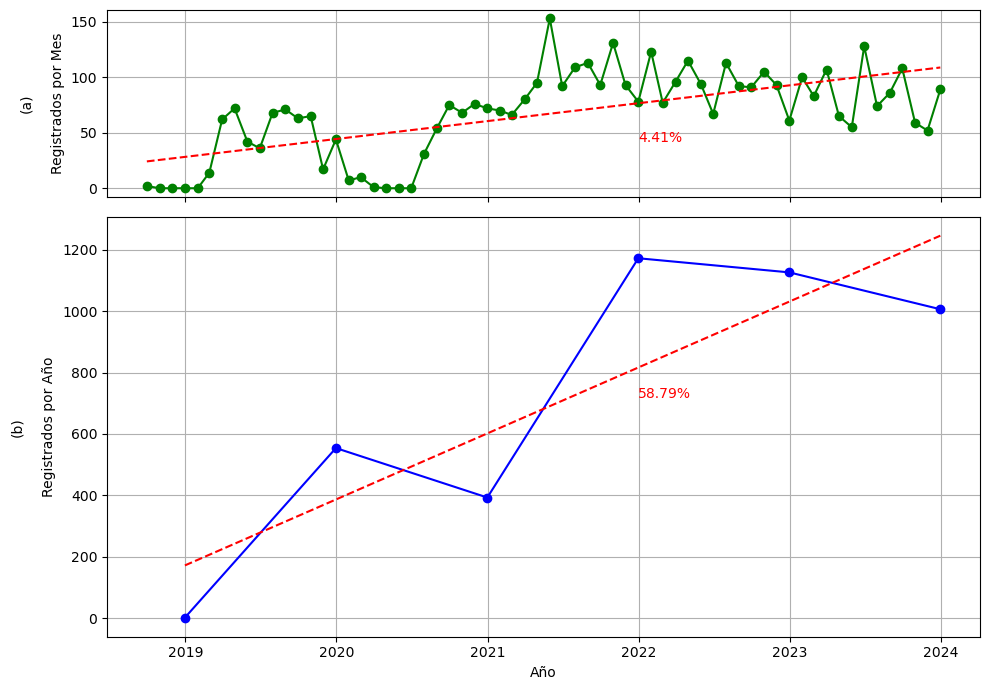
\includegraphics[width=\textwidth, height=.5\textheight]{../images/marcoref/tendencia_profesionales_syso_registrados.png}
        \caption{Registro de profesionales SySO:\\(a) Mensual (b) Anual.}
        \label{fig:profesionales_syso_registrados}
    \end{figure}
    \end{columns} 

    \begin{figure}
      \centering
      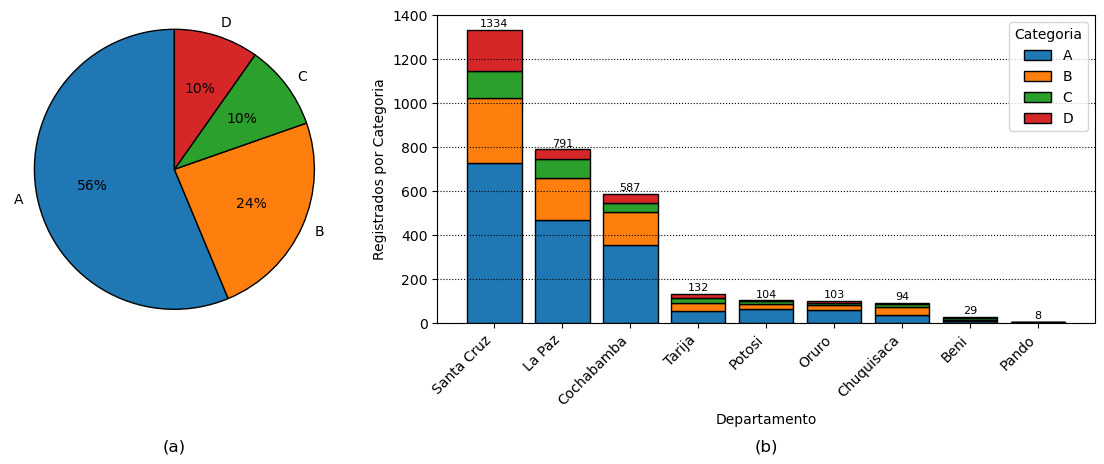
\includegraphics[width=0.9\textwidth]{../images/marcoref/profesionales_syso_por_categoria.png}
      \caption{Profesionales SST activos:\\Distribución de categorías (a) porcentual (b) por departamento.}
      \label{fig:profesionales_syso_por_categoria} 
    \end{figure}
\end{frame}

\begin{frame}{Definición del Problema}
  ¿Cómo desarrollar un software que identifique de manera efectiva los riesgos laborales, facilitando así el desarrollo y la gestión eficiente de un PGSST?
\end{frame}

\begin{frame}{Objetivos}
  \begin{block}{Objetivo general}
  Implementar un sistema automatizado que permita la identificación de riesgos laborales, facilitando el desarrollo y la gestión eficiente de PGSST.
  \end{block}
  \begin{block}{Objetivos específicos}
  \begin{itemize}
  \item Analizar los procesos para desarrollar los documentos solicitados por la NTS-009/23.
  \item Implementar sistema automatizado de detección de riesgo basado en imágenes y descripciones de texto.
  \item Ofrecer la capacidad de generar automáticamente los PGSST requeridos.
  \item Diseñar una interfaz amigable para el uso del software.
  \end{itemize}
  \end{block}
\end{frame}

\begin{frame}{Justificación}
  \begin{block}{Justificación legal}
  La implementación del sistema se fundamenta en la NTS-009/23 y la Ley General de Higiene, Seguridad Ocupacional y Bienestar.
  \end{block}
  \begin{block}{Justificación tecnológica}
  La automatización y la IA ofrecen una oportunidad para mejorar la gestión de la seguridad y salud ocupacional.
  \end{block}
  \begin{block}{Justificación social}
  Mejorar las condiciones de trabajo beneficia a los trabajadores y a la sociedad en general.
  \end{block}
\end{frame}

\begin{frame}{Delimitación}
  \begin{block}{Límites}
  \begin{itemize}
  \item Contenido del software delimitado por requerimientos técnicos y entregables de la NTS-009/23.
  \item El contenido generado debe estar en conformidad con la norma ISO 45001:2018.
  \item El sistema se adherirá a estándares ISO 12207:2017, ISO 25000:2014 y ISO 420001:2023.
  \item El software no automatizará los estudios de higiene, utilizando plantillas para completar y analizar datos recolectados.
  \end{itemize}
  \end{block}
  \begin{block}{Alcances}
  \begin{itemize}
  \item Prototipo funcional de aplicación web y móvil.
  \item Documentación del desarrollo del software.
  \end{itemize}
  \end{block}
\end{frame}

%--------------------------------------------------------------------------------
\section{Marco teórico y legal}

\begin{frame}[allowframebreaks]{Salud y Seguridad Ocupacional}

  \begin{columns}[T] % alinear arriba
    \begin{column}{0.5\textwidth}
      Conceptos Fundamentales
      \begin{itemize}
          \item Seguridad Ocupacional
          \item Salud Ocupacional
          \item Higiene Ocupacional
          \item Enfermedad Ocupacional
          \item Sistema de Gestión de Riesgos Ocupacionales
      \end{itemize}
    \end{column}
    \begin{column}{0.5\textwidth}
      Condiciones de Trabajo
      \begin{itemize}
          \item Iluminación
          \item Estrés Térmico
          \item Sonometría
          \item Ventilación
          \item Señalización
          \item Ergonomía
          \item Equipo de Protección Personal (EPP)
          \item Comité Mixto
          \item Inspección de Salud y Seguridad en el trabajo
      \end{itemize}
    \end{column}
  \end{columns}

  \framebreak

  \begin{columns}[T]
    \begin{column}{0.5\textwidth}
      \begin{itemize}
        \item Accidentes e Incidentes Ocupacionales
        \item Factores de accidentes
        \begin{itemize}
            \item Actos Inseguros
            \item Condición Insegura
        \end{itemize}
        \item Ingeniería de Seguridad
        \item Práctica de Seguridad
        \item Investigación de accidentes
        \item Peligro
      \end{itemize}
      \end{column}
      \begin{column}{0.5\textwidth}
        \begin{itemize}
        \item Riesgo
        \begin{itemize}
            \item Riesgo Físico
            \item Riesgo Mecánico
            \item Riesgo Químico
            \item Riesgo Biológico
            \item Riesgo Psicosocial
            \item Riesgo Ergonómico
            \item Riesgo Aceptable
        \end{itemize}
      \end{itemize}
    \end{column}
  \end{columns}
\end{frame}

\begin{frame}[allowframebreaks]{Legislación Aplicable a la SySO}
  \begin{itemize}
      \item Normativa obligatoria
      \begin{itemize}
          \item Constitución Política del Estado
          \item Ley General del Trabajo
          \item Reglamento de la Ley General de Trabajo
          \item Ley General de Higiene, Seguridad Ocupacional y Bienestar
          \item Disposiciones Complementarias\\ \quad Resolución Ministerial N° 992/23\\ \quad Resolución Ministerial N° 437/22\\ \quad Resolución Ministerial N° 849/14\\ \quad Resolución Ministerial N° 527/09
      \end{itemize}
      \framebreak
      \item Normativa voluntaria
      \begin{itemize}
          \item NB/ISO 62005:2005 - Calidad de Aire
          \item NB/ISO 55001:2005 - Señalización
          \item NB/ISO 51002:2012 - Iluminación
          \item NB/ISO 7243:2018 - Estrés térmico
          \item NB/ISO 45001:2018 - Sistema de Gestión Seguridad y Salud en el Trabajo
          \item NB/ISO 51001:2022 - Ventilación general de los lugares de trabajo
          \item NB/ISO 58005:2022 - Prevención y protección contra incendios
          \item NB/ISO 11226:2022 - Evaluación de posturas de trabajo estáticas
      \end{itemize}
  \end{itemize}
\end{frame}

\begin{frame}[allowframebreaks]{Metodologías de Desarrollo de Software}
  \begin{itemize}
      \item Cascada
  \end{itemize}

  \begin{figure}
    \centering
    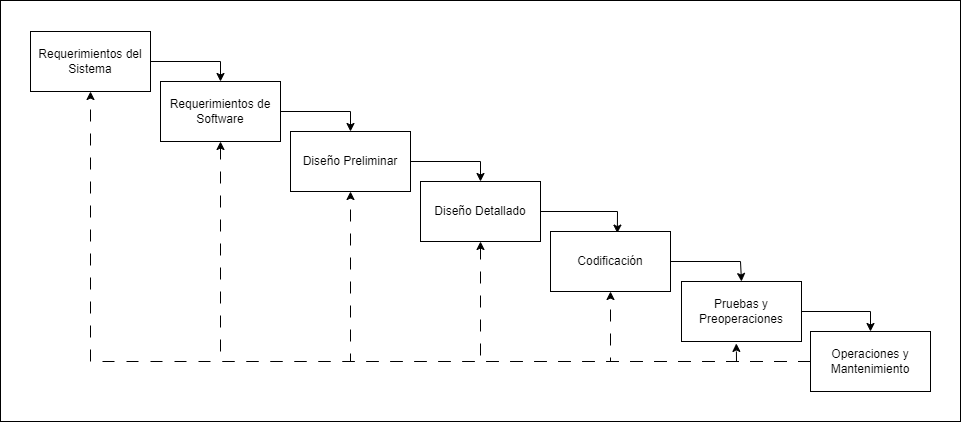
\includegraphics[width=.8\textwidth]{../images/marcoteorico/modelo_cascada.png}
    \caption{Proceso de desarrollo en Cascada.}
      \vspace{-0.2cm}
    \footnotesize{{Elaboración propia a partir de ``\textit{\citefield{auer1990solution}{title}}'' (\citeyear{auer1990solution}).}}
    \label{fig:modelo_desarrollo_cascada} 
  \end{figure}

  \begin{itemize}
      \item Agile
      \begin{itemize}
          \item Programación Extrema
      \end{itemize}
    \end{itemize}
    
    \begin{figure}
      \centering
      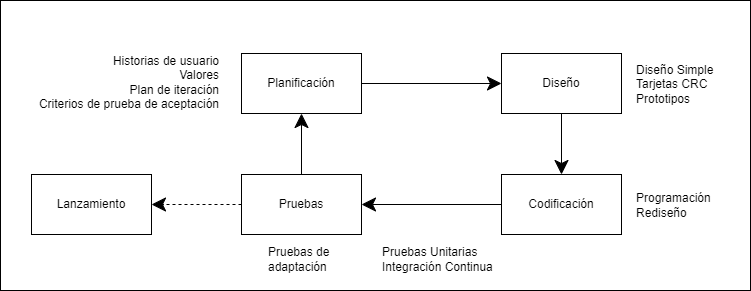
\includegraphics[width=.8\textwidth]{../images/marcoteorico/modelo_xp.png}
      \caption{Proceso de desarrollo bajo la metodología de Programación Extrema.}
        \vspace{-0.2cm}
      \footnotesize{{Elaboración propia a partir de ``\textit{\citefield{pressman2005software}{title}}'' (\citeyear{pressman2005software}).}}
      \label{fig:modelo_desarrollo_xp} 
    \end{figure}

    \begin{itemize}
        \item Scrum
    \end{itemize}

    \begin{figure}
      \centering
      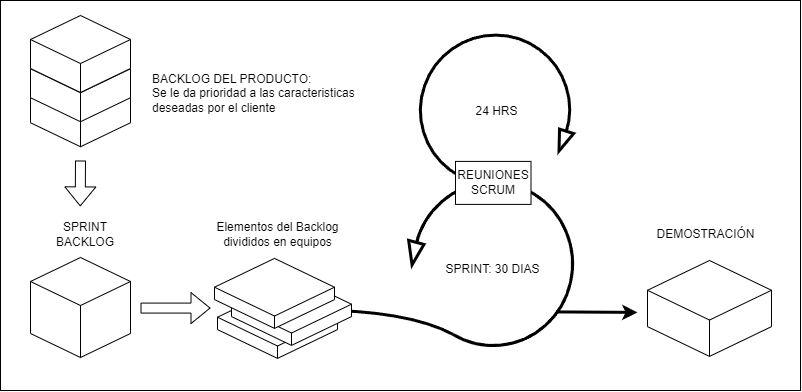
\includegraphics[width=.75\textwidth]{../images/marcoteorico/modelo_scrum.png}
      \caption{Proceso de desarrollo bajo la metodología Scrum.}
        \vspace{-0.2cm}
      \footnotesize{{Elaboración propia a partir de ``\textit{\citefield{pressman2005software}{title}}'' (\citeyear{pressman2005software}).}}
      \label{fig:modelo_desarrollo_scrum} 
    \end{figure}

\end{frame}

\begin{frame}{Análisis y Evaluación de Software}
  \begin{itemize}
      \item Estándar ISO 25000:2014 \\
      \quad \textit{System and Software Quality Requirements and Evaluation}\\
      \quad (Requisitos y Evaluación de la Calidad del Sistema y del Software)
      \item Estándar ISO 12207:2017 \\ 
      \quad \textit{Software life cycle processes} (Procesos del ciclo de vida del software)
      \item Estándar ISO 420001:2023 \\  
      \quad \textit{Artificial intelligence Management system}\\ 
      \quad(Sistema de Gestión de Inteligencia Artificial)
  \end{itemize}
\end{frame}

\begin{frame}[allowframebreaks]{Inteligencia Artificial}

  \begin{figure}[htb]
    \centering
    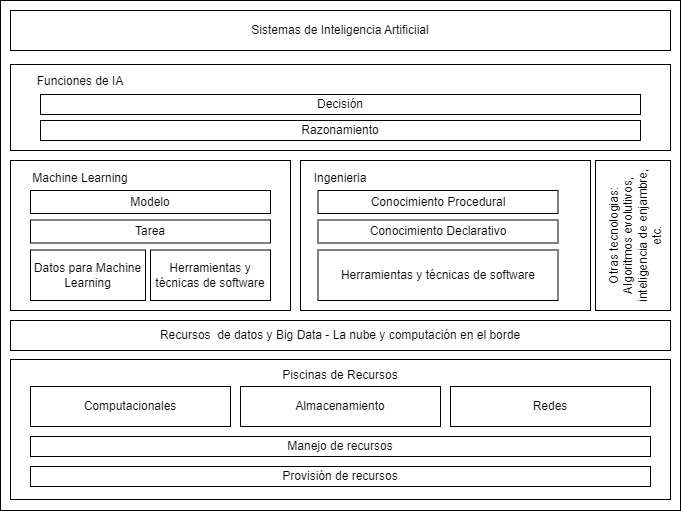
\includegraphics[height=.6\textheight]{../images/marcoteorico/ai_ecosystem.png}
    \caption{Ecosistema de un sistema de inteligencia artificial.}
      \vspace{-0.2cm}
    \footnotesize{{Elaboración propia a partir de ``\textit{\citefield{iso22989}{title}}'' (\citeyear{iso22989}).}}
    \label{fig:ai_ecosystem} 
  \end{figure}

  Aprendizaje \footnotemark
  \begin{itemize}
      \item Sistemas basados en heurística
      \item Sistemas basados en aprendizaje automático
  \end{itemize}

  \footnotetext[1]{Entre algunas bases de datos útiles se identificaron BINVAC, BASEMAQ y BASEQUIM.} 

\end{frame}

\section{Referencias}
\begin{frame}[allowframebreaks]{Referencias}
  \printbibliography
\end{frame}

\end{document}